\documentclass[conference]{IEEEtran}

\makeatletter
\def\ps@IEEEtitlepagestyle{%
  \def\@oddfoot{\mycopyrightnotice}%
  \def\@evenfoot{}%
}
\def\mycopyrightnotice{%
{\footnotesize XXX-X-XXXX-XXXX-X/XX/\$XX.00~\copyright~20XX IEEE\hfill}%
  \gdef\mycopyrightnotice{}
}
\makeatother

\IEEEoverridecommandlockouts

\usepackage{cite}
\usepackage{amsmath,amssymb,amsfonts}
\usepackage{graphicx}
\usepackage{textcomp}
\usepackage{xcolor}
\usepackage{url}
\usepackage{booktabs}

\usepackage{eso-pic}
\newcommand\AtPageUpperMyright[1]{\AtPageUpperLeft{%
 \put(\LenToUnit{0.17\paperwidth},\LenToUnit{-2cm}){%
     \parbox{0.9\textwidth}{\raggedleft\fontsize{8}{11}\selectfont #1}}%
}}
\newcommand{\conf}[1]{%
\AddToShipoutPictureBG*{%
\AtPageUpperMyright{#1}
}
}

\begin{document}

\title{\vspace*{1cm} A Japanese-Human-Grounded Benchmark for Literary Emotion Understanding with Multilingual Robustness Tests}

\author{
\IEEEauthorblockN{Naruki Shirahama}
\IEEEauthorblockA{\textit{Shimonoseki City University} \\
Shimonoseki, Yamaguchi, Japan \\
nshirahama@ieee.org}
\and
\IEEEauthorblockN{Yuma Yoshimoto}
\IEEEauthorblockA{\textit{NIT (KOSEN), Kitakyushu College} \\
Kitakyushu, Fukuoka, Japan \\
yoshimoto@kct.ac.jp}
\and
\IEEEauthorblockN{Naofumi Nakaya}
\IEEEauthorblockA{\textit{Juntendo University} \\
Urayasu, Chiba, Japan \\
n.nakaya.ac@juntendo.ac.jp}
\and
\IEEEauthorblockN{Junji Nishino}
\IEEEauthorblockA{\textit{Tamagawa University} \\
Machida, Tokyo, Japan \\
nishinojunji@eng.tamagawa.ac.jp}
\and
\IEEEauthorblockN{Satoshi Watanabe}
\IEEEauthorblockA{\textit{Shizuoka Institute of Science and Technology} \\
Fukuroi, Shizuoka, Japan \\
satoshi\_watanabe@ieee.org}
}

\maketitle
\conf{\textit{Proc. of the International Conference on Electrical, Computer, Communications and Mechatronics Engineering (ICECCME 2026) \\ 15--17 October 2026, Bali, Indonesia}}

\begin{abstract}
Human-grounded validation remains a central gap in large language model (LLM) evaluation for affective text understanding. Existing benchmarks and multilingual profiling can reveal model-to-model or language-to-language variation, but such variation alone does not show which systems are closest to human judgments. This paper proposes a compact human-grounded multilingual benchmark for literary emotion evaluation using three Japanese literary works and four continuous affect dimensions: interest, surprise, sadness, and anger. Japanese Visual Analogue Scale (VAS) ratings from student readers define the reference profile, and six contemporary LLMs are compared through a unified multi-provider experimental platform. The primary endpoint is alignment with the Japanese human reference under a neutral-reader prompt; English and Chinese conditions are treated as robustness tests for cross-language drift, not as co-equal human-grounded endpoints. Claude Sonnet 4.5 achieved the lowest mean absolute error to the Japanese human reference (20.026), whereas Gemini 2.5 Pro showed the largest error (28.952). GPT-5.4 achieved the strongest rank-order agreement with the human profile, while Qwen3.6 Plus and GPT-5.4 exhibited the smallest average cross-language drift (3.346 and 3.354, respectively). The results show that primary human alignment and multilingual robustness are related but separable properties, making the benchmark suitable for compact and reproducible model screening.
\end{abstract}

\begin{IEEEkeywords}
large language models, human-grounded evaluation, literary emotion understanding, multilingual robustness, visual analogue scale
\end{IEEEkeywords}

\section{Introduction}
LLM evaluation for affective text understanding increasingly includes benchmark suites, multilingual tests, and human--AI comparisons. These approaches are valuable, but they often leave a critical endpoint hierarchy under-specified: model-to-model or language-to-language variation can show that outputs differ, but it cannot show whether those outputs are close to human judgments. Smaller human-versus-AI comparisons, in turn, often focus on a single model or a single language condition \cite{shirahama2025vas,paech2024eqbench,huang2024emotionbench}. A compact benchmark is therefore useful only if it keeps the human reference explicit and does not treat multilingual stability as a substitute for human validity.

This paper addresses that gap by using Japanese Visual Analogue Scale (VAS) human ratings as the reference profile and treating the Japanese condition as the primary endpoint. English and Chinese are analyzed only as robustness conditions for cross-language drift. The contribution is therefore not a generic language-effect study, but a compact human-grounded framework that separates primary Japanese human alignment from secondary-language robustness.

The present paper makes three concrete contributions. First, it provides a reproducible benchmark design that keeps the primary claim tightly anchored to Japanese human reference data. Second, it separates human alignment from multilingual robustness so that secondary-language behavior is not over-interpreted as a substitute for human validity. Third, it offers a two-axis screening view---Japanese calibration versus cross-language drift---that is practical for compact engineering evaluation before larger multilingual or multi-persona studies are undertaken.

\section{Related Work}
The present study sits at the intersection of four lines of work. The first compares human and AI emotion judgments and motivates the use of continuous scales rather than coarse categorical labels. Our earlier VAS-versus-Likert study showed that a VAS-based design is practical for short-story affect evaluation and provides a stronger foundation for fine-grained human--LLM comparison than a small discrete scale \cite{shirahama2025vas}.

The second line concerns benchmark design for LLM emotional intelligence. Benchmark suites such as EQ-Bench, EmotionBench, EmoBench, and EmotionQueen have helped standardize evaluation of emotional reasoning, empathy, and affective response quality \cite{paech2024eqbench,huang2024emotionbench,sabour2024emobench,chen2024emotionqueen}. However, these suites are not primarily designed to ask which current models are closest to a human reference profile on a literary reading task with continuous story-by-emotion scoring.

The third line concerns multilingual and robustness-oriented LLM evaluation. Language changes can alter lexical choice, narrative framing, and calibration, so multilingual comparison is necessary when a benchmark is meant to support deployment across translated conditions. Yet multilingual variation alone is not equivalent to human validity unless matched human references are also available.

The fourth line is our own prior platform-development and mathematical-characterization work. Those studies established that LLMs differ substantially in reliability, controllability, and emotional individuality across a broad model landscape \cite{openrouterplatform,shirahama2026mdpi}. The present paper intentionally narrows the design: one neutral-reader primary condition, one human-grounded language endpoint, and multilingual runs interpreted as robustness analyses rather than as direct substitutes for human validation.

\section{Data and Methods}
\textbf{Human reference data.} The benchmark uses respondent-level VAS data for three short Japanese literary texts and four affect dimensions: interest, surprise, sadness, and anger. The three works are Kyusaku Yumeno's \textit{The Pocket Watch} (T1; \textit{Kaichu dokei}), Kyusaku Yumeno's \textit{The Money and the Pistol} (T2; \textit{Okane to pisutoru}), and Kotaro Takamura's \textit{The Tattered Ostrich} (T3; \textit{Boroboro na dacho}). The task was administered in Japanese to student readers as a VAS survey in which each respondent rated the three texts on the same four emotions after reading each work. Ninety-one human responses were collected, of which 86 were complete cases retained for the primary aggregate reference profile. The public repository stores only sanitized numeric derivatives. The present analysis reuses only anonymized secondary numeric derivatives of the student VAS data; raw survey exports and platform metadata are not redistributed.

\textbf{Texts and model panel.} The computational benchmark evaluates the same three works used in the human task and compares six contemporary LLMs from six major providers: Claude Sonnet 4.5, GPT-5.4, Grok 4.20, Qwen3.6 Plus, DeepSeek V3.2, and Gemini 2.5 Pro. Each model was queried in Japanese, English, and Chinese. The model panel was intentionally kept compact to match the engineering-pilot scope of the paper while preserving vendor diversity.

\textbf{Task definition.} The neutral-reader model run operationalized the same four affect dimensions on a 0--100 scale to approximate the human VAS task. One LLM experimental unit consisted of one model, one language, one text, one neutral-reader prompt, and one repetition. The model received the full literary text, the neutral-reader role, the four emotion definitions, and the scoring rule that 0 means the emotion is not felt at all, 50 means moderately felt, and 100 means extremely strongly felt. It returned one JSON object containing four integer scores and brief text-grounded reasons. A single neutral-reader prompt was used in all languages so that the benchmark would remain interpretable as a human-alignment pilot rather than collapse back into persona-conditioned evaluation. Japanese human alignment is the primary endpoint because the reference VAS data were collected in Japanese, with Japanese source texts and Japanese task instructions used in the primary human--LLM alignment condition. English and Chinese are therefore not treated as co-equal human-grounded evaluations but as cross-language robustness tests; in those runs, both the literary texts and the task instructions were language-matched using fixed author-prepared translations, so drift reflects the combined effect of translated text and prompt language rather than instruction language alone. Because the benchmark is intentionally compact, the analysis is interpreted descriptively for screening utility rather than formal significance testing. This design keeps persona-conditioned prompting outside the center of the present paper, because persona and temperature were confounded in our earlier LLM-only design \cite{shirahama2026mdpi}.

\begin{figure*}[t]
\centering
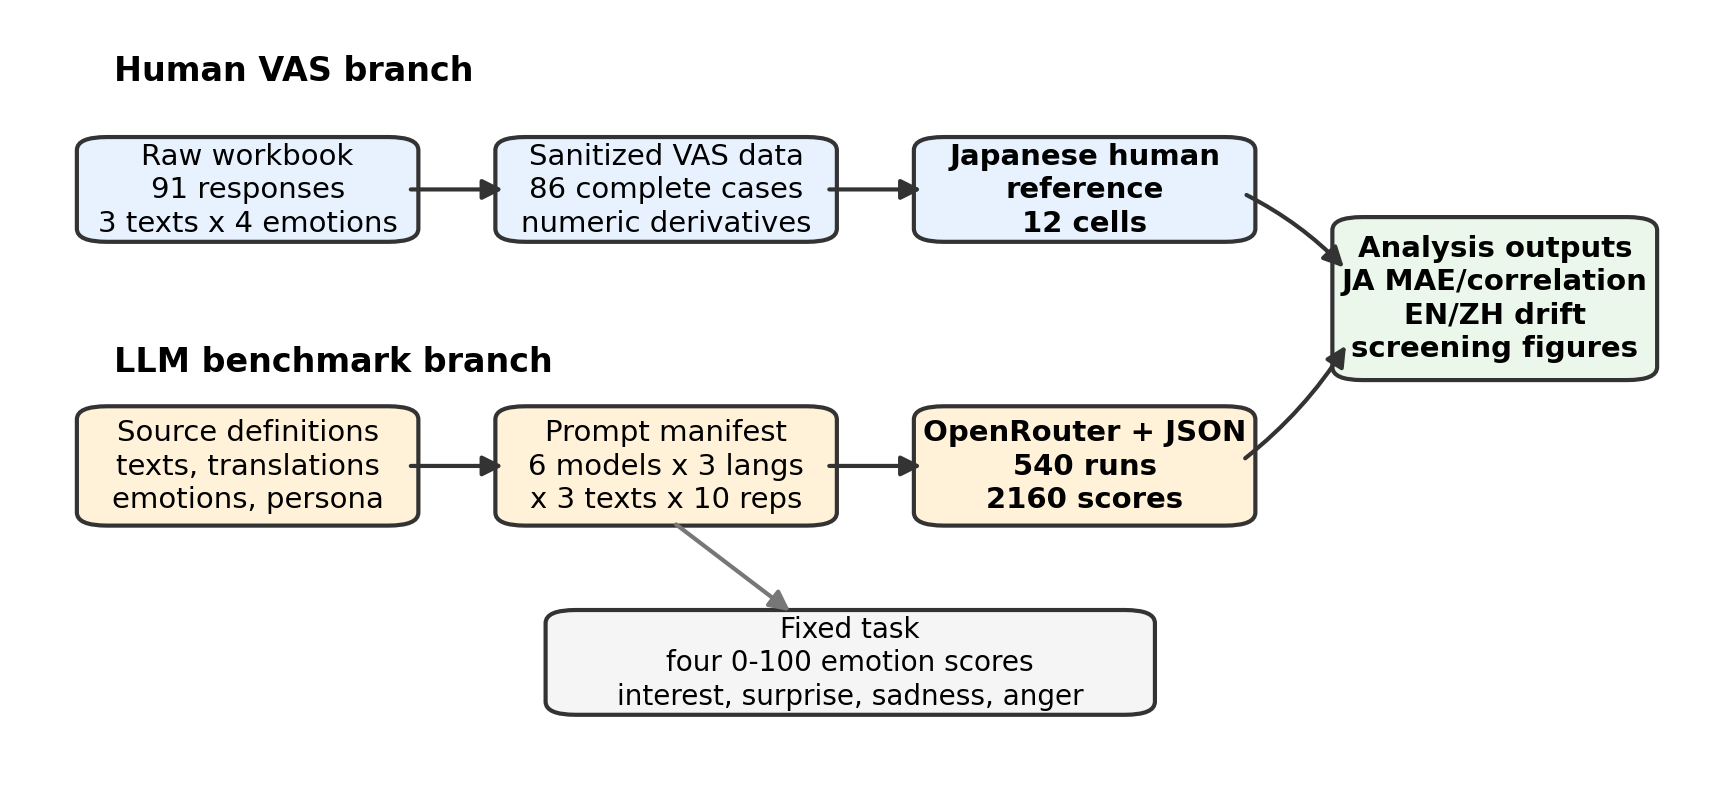
\includegraphics[width=0.96\textwidth]{fig/figure1_system_workflow.pdf}
\caption{System configuration and data flow for the benchmark. The human branch converts the private Japanese VAS workbook into sanitized story-by-emotion reference cells. The LLM branch combines the fixed source definitions, translated texts, prompt template, response schema, and model manifest to run the neutral-reader benchmark through OpenRouter. The analysis compares Japanese model profiles with the human reference and treats English and Chinese as cross-language robustness conditions.}
\label{fig:workflow}
\end{figure*}

\textbf{Aggregation.} Let $s \in \{1,2,3\}$ index texts and $d \in \{1,2,3,4\}$ index affect dimensions. The Japanese human reference profile is
\begin{equation}
H_{s,d}=\frac{1}{N_s}\sum_{i=1}^{N_s} y_{i,s,d},
\end{equation}
where $y_{i,s,d}$ is the VAS score from respondent $i$ and $N_s$ is the number of complete human responses for text $s$. For model $m$, language $\ell \in \{\mathrm{JA},\mathrm{EN},\mathrm{ZH}\}$, and repetition count $R=10$, the aggregated model profile is
\begin{equation}
M_{m,\ell,s,d}=\frac{1}{R}\sum_{r=1}^{R} x_{m,\ell,s,d,r}.
\end{equation}
This yields a 12-value story-by-emotion profile for each model-language condition.

\textbf{Metrics.} The primary endpoint is Japanese human alignment. For each model, Japanese scores were aggregated to a story-by-emotion profile and compared against the Japanese human reference using mean absolute error (MAE), Pearson correlation, and Spearman rank correlation:
\begin{equation}
\mathrm{MAE}_{m,\mathrm{JA}}=\frac{1}{12}\sum_{s,d}\left|M_{m,\mathrm{JA},s,d}-H_{s,d}\right|.
\end{equation}
English and Chinese were not treated as additional human-grounded endpoints. Instead, cross-language drift was defined as the mean absolute difference between each model's English or Chinese story-by-emotion score profile and the same model's Japanese profile:
\begin{equation}
D_{m,\ell}=\frac{1}{12}\sum_{s,d}\left|M_{m,\ell,s,d}-M_{m,\mathrm{JA},s,d}\right|,~~ \ell \in \{\mathrm{EN},\mathrm{ZH}\}.
\end{equation}
We also report the average drift
\begin{equation}
\bar{D}_m=\frac{D_{m,\mathrm{EN}}+D_{m,\mathrm{ZH}}}{2}.
\end{equation}
Lower MAE and lower drift are better. Because the benchmark is intentionally compact, the paper emphasizes descriptive comparison and screening utility rather than formal significance testing.

\textbf{Protocol and reproducibility.} The protocol comprised 91 human responses, with 86 complete cases retained for the primary aggregate reference profile, across 3 texts and 4 affect dimensions. The model side covered 6 models $\times$ 3 languages $\times$ 3 texts $\times$ 10 repetitions under one neutral-reader prompt, yielding 540 neutral-reader model runs and 2160 numeric scores. Figure~\ref{fig:workflow} summarizes the two data branches and the downstream analysis. For reproducibility, the public repository stores only sanitized numeric derivatives of the student VAS data, while raw survey exports and platform metadata are not redistributed.

\begin{table}[t]
\caption{Primary benchmark design summary.}
\label{tab:design}
\centering
\begin{tabular}{lr}
\toprule
Item & Value \\
\midrule
Human responses & 91 \\
Complete cases & 86 \\
Texts & 3 \\
Affect dimensions & 4 \\
Models & 6 \\
Languages & 3 (JA/EN/ZH) \\
Prompt condition & 1 (neutral reader) \\
Repetitions per condition & 10 \\
Total neutral-reader model runs & 540 \\
Total numeric scores & 2160 \\
\bottomrule
\end{tabular}
\end{table}

\section{Results}
Figure~\ref{fig:workflow} summarizes the system configuration and data flow, Table~\ref{tab:design} summarizes the benchmark design, Figure~\ref{fig:ja-ranking} shows the Japanese human-alignment ranking, Figure~\ref{fig:drift} shows cross-language drift relative to Japanese, Table~\ref{tab:primary} reports the core summary statistics, and Figure~\ref{fig:tradeoff} visualizes the two-axis screening view.

\textbf{Japanese human alignment.} In the primary Japanese condition, Claude Sonnet 4.5 achieved the lowest mean absolute error (MAE) to the human reference (20.026), followed by DeepSeek V3.2 (20.100), Qwen3.6 Plus (20.744), GPT-5.4 (21.113), and Grok 4.20 (21.410), whereas Gemini 2.5 Pro showed the largest error (28.952). The spread between the best and worst models was therefore 8.926 points. At the same time, the top four models were tightly clustered within only 1.087 MAE points, indicating that model screening would be sensitive to relatively small calibration differences within the stronger half of the panel.

\begin{figure*}[t]
\centering
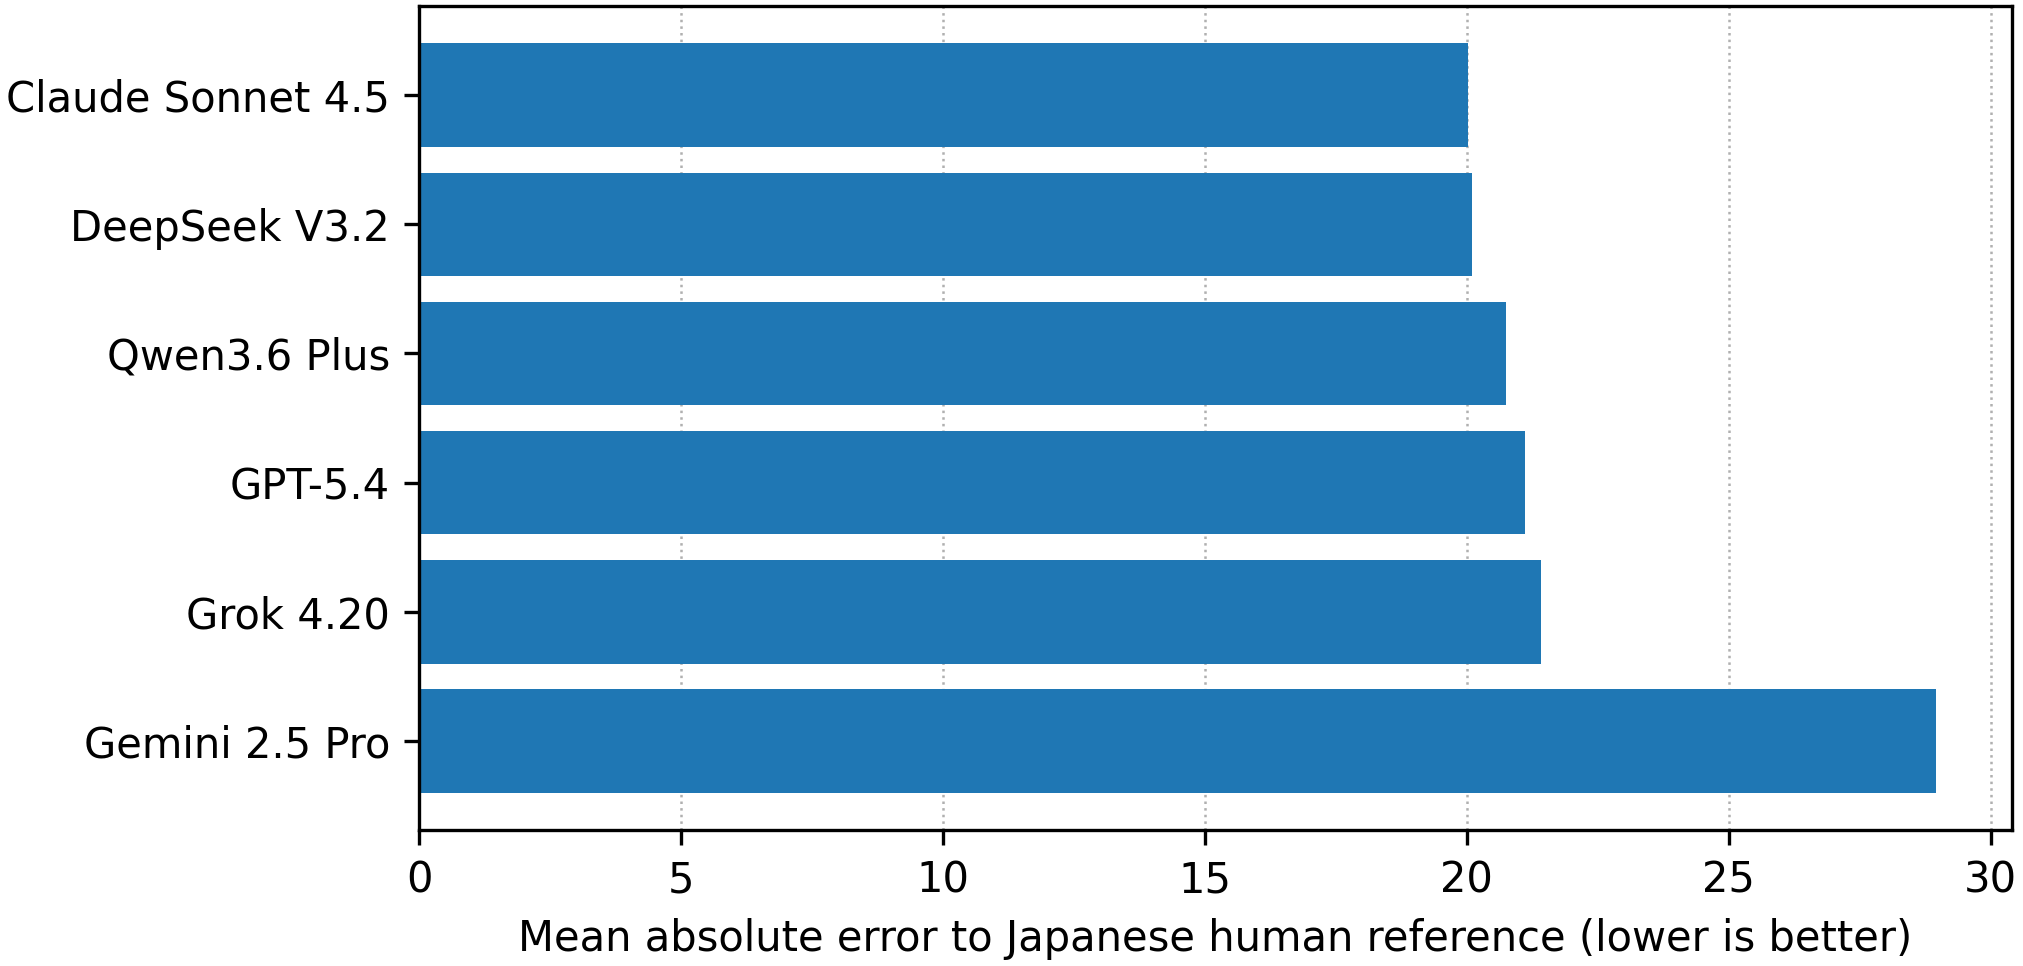
\includegraphics[width=0.94\textwidth]{fig/figure2_ja_ranking.pdf}
\caption{Japanese human-alignment ranking of the six selected models under the neutral-reader condition. Models are ordered by mean absolute error (MAE) to the Japanese human reference; lower values indicate closer agreement with human VAS judgments. Correlation coefficients are reported separately in Table~\ref{tab:primary}.}
\label{fig:ja-ranking}
\end{figure*}

GPT-5.4 yielded both the highest Pearson correlation with the Japanese human profile ($r = 0.475$) and the highest Spearman rank correlation ($\rho = 0.441$). This split is important because absolute calibration and rank-order agreement should be distinguished rather than collapsed into a single score. Claude Sonnet 4.5 was the closest in absolute intensity level, whereas GPT-5.4 best preserved relative ordering across the 12 human-reference cells.

\textbf{Cross-language robustness.} For cross-language robustness, Qwen3.6 Plus exhibited the smallest average drift relative to Japanese ($\bar{D}=3.346$), followed closely by GPT-5.4 ($\bar{D}=3.354$) and Gemini 2.5 Pro ($\bar{D}=4.729$). By contrast, DeepSeek V3.2 showed the largest average drift ($\bar{D}=6.396$), with the largest single-language drift observed in its English condition (7.875). Across all models and secondary languages, drift ranged from 2.983 to 7.875 points.

\begin{figure*}[t]
\centering
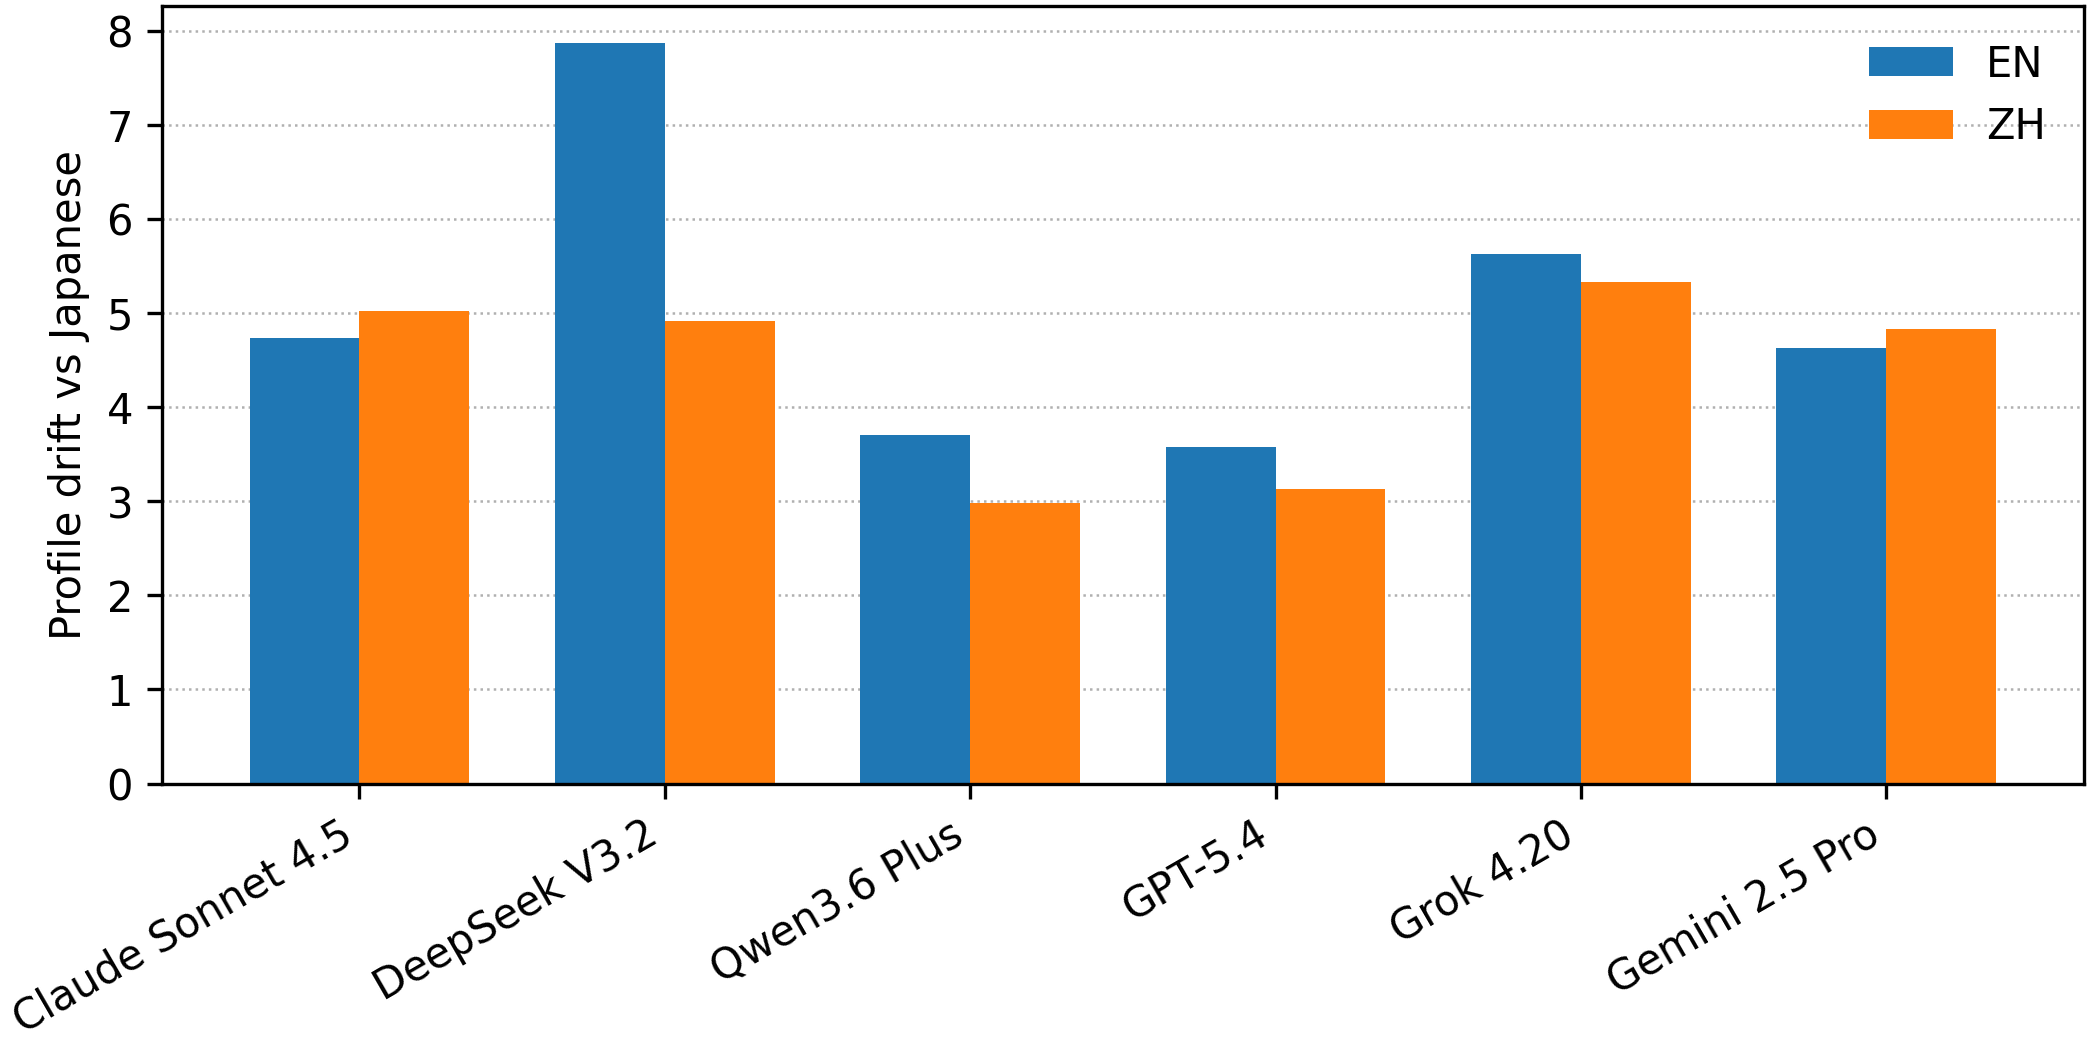
\includegraphics[width=0.94\textwidth]{fig/figure3_cross_language_drift.pdf}
\caption{Cross-language drift relative to Japanese for the six selected models under the neutral-reader condition. Drift is defined as the mean absolute difference between a model's English or Chinese story-by-emotion score profile and the same model's Japanese profile. Smaller values indicate greater cross-language robustness.}
\label{fig:drift}
\end{figure*}

The English condition was slightly less stable on average than the Chinese condition in this six-model panel: mean English drift was 5.024, whereas mean Chinese drift was 4.371. That difference is descriptive rather than inferential, but it still shows why robustness should not be assumed to be symmetric across translated conditions.

\begin{table*}[t]
\caption{Primary quantitative summary of Japanese human alignment and cross-language drift for the six selected models.}
\label{tab:primary}
\centering
\small
\begin{tabular}{lrrrrrr}
\toprule
Model & JA MAE & JA Pearson $r$ & JA Spearman $\rho$ & EN drift & ZH drift & Avg drift \\
\midrule
Claude Sonnet 4.5 & 20.026 & 0.442 & 0.252 & 4.733 & 5.025 & 4.879 \\
DeepSeek V3.2 & 20.100 & 0.459 & 0.301 & 7.875 & 4.917 & 6.396 \\
Qwen3.6 Plus & 20.744 & 0.374 & 0.214 & 3.708 & 2.983 & 3.346 \\
GPT-5.4 & 21.113 & 0.475 & 0.441 & 3.575 & 3.133 & 3.354 \\
Grok 4.20 & 21.410 & 0.305 & 0.112 & 5.625 & 5.333 & 5.479 \\
Gemini 2.5 Pro & 28.952 & 0.261 & 0.112 & 4.625 & 4.833 & 4.729 \\
\bottomrule
\end{tabular}
\end{table*}

\textbf{Two-axis screening view.} The Japanese ranking and the drift ranking are related but not identical. Claude Sonnet 4.5 is the best-calibrated model in Japanese, whereas Qwen3.6 Plus shows the smallest average cross-language drift. Gemini 2.5 Pro has the largest Japanese MAE, while DeepSeek V3.2 has the largest average drift. Figure~\ref{fig:tradeoff} makes this separation explicit by plotting Japanese human-alignment MAE against average EN/ZH drift.

\begin{figure}[t]
\centering
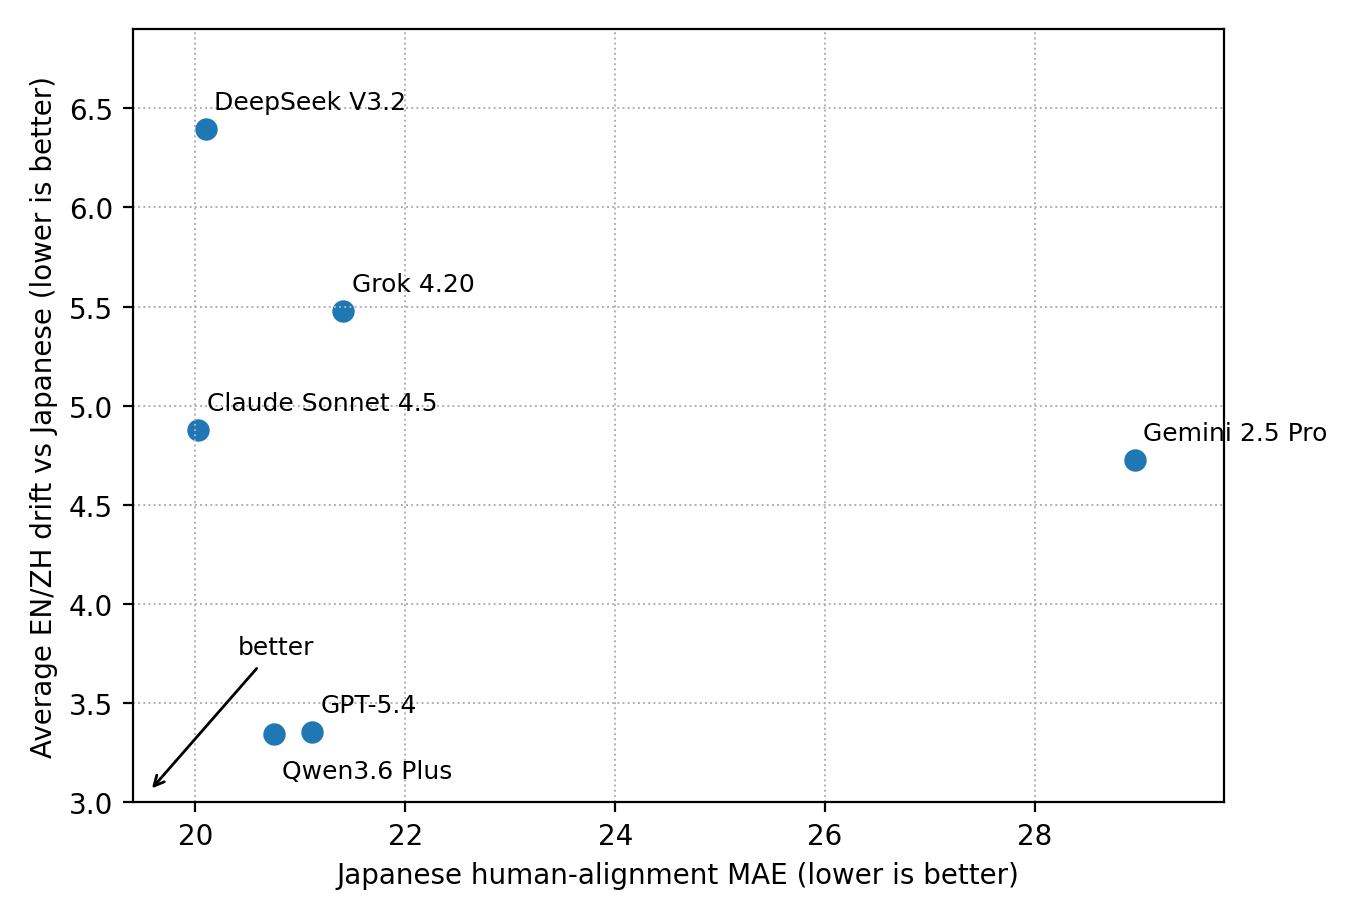
\includegraphics[width=0.98\columnwidth]{fig/figure4_alignment_vs_avg_drift.pdf}
\caption{Two-axis screening view of the benchmark. The horizontal axis shows Japanese human-alignment MAE and the vertical axis shows average EN/ZH drift relative to Japanese. The lower-left region is preferable when both primary-language calibration and multilingual robustness matter.}
\label{fig:tradeoff}
\end{figure}

No single model dominates both axes. Claude Sonnet 4.5 is strongest on the primary human-grounded endpoint, Qwen3.6 Plus and GPT-5.4 are strongest on multilingual stability, and Gemini 2.5 Pro shows that moderate robustness does not compensate for weak primary-language alignment. This separation is important for deployment-oriented evaluation: a model may align relatively well with human intensity levels in the primary language while showing different stability under translation, or vice versa.

\section{Discussion}
Three points follow from these results. First, multilingual variation is not the same as human validity. A model can look plausible under multilingual prompting yet still diverge substantially from the Japanese human reference when calibration is evaluated directly. This is the main reason we treat Japanese human alignment as the primary endpoint and EN/ZH behavior as robustness analysis rather than as co-equal human-grounded evaluation.

Second, a compact benchmark can still produce operationally useful screening information. In the primary Japanese condition, Claude Sonnet 4.5 achieved the lowest MAE to the human reference (20.026), and the top four models were separated by only 1.087 MAE points. GPT-5.4 instead yielded the highest Japanese Pearson and Spearman correlations (0.475 and 0.441), indicating that absolute calibration and rank-order agreement should be distinguished rather than collapsed into a single score. For multilingual robustness, Qwen3.6 Plus and GPT-5.4 showed the smallest average EN/ZH drift (3.346 and 3.354), whereas DeepSeek V3.2 showed the largest average drift (6.396). No single model therefore dominates both human alignment and multilingual robustness.

\begin{table}[t]
\caption{Practical screening interpretation of the six-model panel.}
\label{tab:screening}
\centering
\scriptsize
\begin{tabular}{@{}p{0.24\columnwidth}p{0.30\columnwidth}p{0.29\columnwidth}@{}}
\toprule
Model & Strength & Caution \\
\midrule
Claude Sonnet 4.5 & Best Japanese MAE & Only mid-level average multilingual drift \\
DeepSeek V3.2 & Second-best Japanese MAE & Largest average drift; English especially unstable \\
Qwen3.6 Plus & Lowest average EN/ZH drift & Japanese alignment below the top two models \\
GPT-5.4 & Highest Japanese Pearson and Spearman; near-best average drift & Not the lowest Japanese MAE \\
Grok 4.20 & Mid-range on both axes & No leading metric in the six-model panel \\
Gemini 2.5 Pro & Moderate average drift & Largest Japanese MAE in the panel \\
\bottomrule
\end{tabular}
\end{table}

Table~\ref{tab:screening} summarizes the same point in operational terms. The benchmark does not identify a single dominant model; instead, it exposes which trade-off each model is making in a compact and reviewable form. That makes the protocol useful for early-stage model narrowing before a larger validation campaign is launched.

Third, the paper clarifies how this ICECCME contribution differs from our earlier LLM-only framework paper. The previous study was designed to characterize emotional individuality under persona-assigned temperatures across a broad 36-model landscape \cite{shirahama2026mdpi}. The present paper instead fixes a neutral-reader primary condition and uses human alignment as the primary endpoint. This shift makes the paper more appropriate for a compact engineering conference contribution focused on benchmark design and cross-language robustness rather than on multidimensional individuality analysis.

This neutral-reader constraint is methodological, not merely stylistic. Once role-playing or creativity prompts are introduced, it becomes harder to know whether score changes reflect better human alignment, a different interpretive stance, or prompt-induced variance. For a human-grounded pilot benchmark, anchoring the main endpoint to one neutral condition makes the comparison easier to interpret and reproduce across providers. Richer persona-conditioned evaluation remains worthwhile, but it should be layered onto a stable human-reference baseline rather than replacing it.

The benchmark should be understood as a stage-1 filter rather than as a deployment certificate. Its main limitations are that it uses only three texts, one Japanese student-reader reference condition, and one neutral-reader primary run. English and Chinese are robustness conditions rather than human-grounded endpoints, and the measured drift reflects both translated literary texts and language-matched task instructions rather than instruction language alone. The analysis is descriptive for screening utility rather than formal significance testing. Provider-compatibility adjustments were also required at the transport/schema layer during data collection, although the task definition, source texts, and scoring dimensions were kept fixed. The next steps are to layer new evidence in a controlled order: more texts, larger human reference samples, and matched human references for English and Chinese.

\section{Conclusion}
This paper presents a compact human-grounded multilingual benchmark for literary emotion evaluation in contemporary large language models. Using a Japanese VAS reference from student readers, we compared six current models under a neutral-reader prompt and found that Claude Sonnet 4.5 achieved the closest absolute agreement with the Japanese human profile, GPT-5.4 achieved the strongest rank-order agreement, and Qwen3.6 Plus achieved the smallest average cross-language drift. More broadly, the results show that primary human alignment and multilingual robustness are related but separable properties. We therefore recommend reporting them independently in future LLM emotion-evaluation studies and using compact human-grounded benchmarks as an initial screening step before larger multilingual or multi-persona evaluations.

\section*{Acknowledgment}
This paper uses a compact human-grounded benchmark design developed within the broader EQ-Fuzzy research program. The authors thank the student readers in the Japanese VAS study and acknowledge the use of Aozora Bunko texts as experimental stimuli.

This work was partially supported by JSPS Grants-in-Aid for Scientific Research (JSPS KAKENHI), Grant Number 26K14983 and 24K13350.

\IEEEtriggeratref{5}
\begin{thebibliography}{00}

\bibitem{shirahama2025vas}
N. Shirahama, N. Nakaya, S. Watanabe, et al., ``Assessing Emotional Intelligence in AI: Visual Analogue Scale vs. Likert Scale in Short Story Comprehension,'' \emph{Journal of the Institute of Industrial Applications Engineers}, vol. 13, no. 1, pp. 21--31, 2025.

\bibitem{shirahama2026mdpi}
N. Shirahama, Y. Yoshimoto, N. Nakaya, and S. Watanabe, ``Mathematical Framework for Characterizing Emotional Individuality in Large Language Models: Temperature Control, Fuzzy Entropy, and Persona-Based Diversity Analysis,'' \emph{Mathematics}, vol. 14, no. 7, Art. no. 1224, 2026.

\bibitem{paech2024eqbench}
S. J. Paech, ``EQ-Bench: An Emotional Intelligence Benchmark for Large Language Models,'' arXiv:2312.06281, 2024.

\bibitem{huang2024emotionbench}
J. Huang, M. H. Lam, E. J. Li, S. Ren, W. Wang, W. Jiao, Z. Tu, and M. R. Lyu, ``Emotionally Numb or Empathetic? Evaluating How LLMs Feel Using EmotionBench,'' arXiv:2308.03656, 2024.

\bibitem{sabour2024emobench}
S. Sabour, S. Liu, Z. Zhang, J. Liu, J. Zhou, A. Sunaryo, T. M. C. Lee, R. Mihalcea, and M. Huang, ``EmoBench: Evaluating the Emotional Intelligence of Large Language Models,'' in \emph{Proc. 62nd Annual Meeting of the Association for Computational Linguistics (ACL)}, 2024, pp. 5986--6004.

\bibitem{chen2024emotionqueen}
Y. Chen, S. Yan, S. Liu, Y. Li, and Y. Xiao, ``EmotionQueen: A Benchmark for Evaluating Empathy of Large Language Models,'' in \emph{Findings of the Association for Computational Linguistics: ACL 2024}, 2024, pp. 2149--2176.

\bibitem{openrouterplatform}
N. Shirahama, N. Nakaya, and S. Watanabe, ``Development of an Experimental Platform for Evaluating LLM Emotion Understanding,'' \emph{ICIC Express Letters}, vol. 20, pp. 191--198, 2026.

\end{thebibliography}

\end{document}
